\documentclass[hyperref={pdfpagelabels=false, unicode},pdf,slideColor,fyma,9pt]{beamer}
\usepackage[utf8]{inputenc}		%kodovani zdrojoveho textu
\usepackage[english]{babel} 		%cestina
\usepackage[IL2]{fontenc}		%font vyladeny pro cestinu
\usepackage{lmodern}			%odstraneni varovani pro IL2
\usepackage{graphicx}
\usepackage{color}
\usepackage{multirow}
\usepackage{subfigure}

% \usepackage[UKenglish]{isodate}

\newcommand\myqt[1]{\quotedblbase #1\textquotedblleft}

%cislovani stran:



\mode<presentation> {
  \usetheme{Boadilla}
	\usecolortheme{default}

  %\setbeamercovered{Berlin beaver default}
	%\setbeamertemplate{navigation symbols}{} % To remove the navigation symbols from the bottom of all slides uncomment this line
%\setbeamertemplate{headline}{}
}

\makeatother
\setbeamertemplate{footline}
{
  \leavevmode%
  \hbox{%
  \begin{beamercolorbox}[wd=.3\paperwidth,ht=2.25ex,dp=1ex,center]{author in head/foot}%
    \usebeamerfont{author in head/foot}\insertshortauthor
  \end{beamercolorbox}%
  \begin{beamercolorbox}[wd=.6\paperwidth,ht=2.25ex,dp=1ex,center]{title in head/foot}%
    \usebeamerfont{title in head/foot}\insertshorttitle\hspace*{3em}
  \end{beamercolorbox}}%
  \begin{beamercolorbox}[wd=.1\paperwidth,ht=2.25ex,dp=1ex,center]{date in head/foot}%
    \insertframenumber{} / \inserttotalframenumber\hspace*{1ex}
  \end{beamercolorbox}%
  \vskip0pt%
}
\makeatletter
\setbeamertemplate{navigation symbols}{}


\title{Performance Testing and Analysis of Qpid-Dispatch Router}
% \subtitle{Master Thesis}
\author[Bc. Jakub Stejskal]{Bc. Jakub Stejskal}
\institute[]{Faculty of Information Technology}
\date[]{\today}

\begin{document}
		\begin{frame}
				\titlepage
        \begin{figure}[ht]
        	\begin{center}
        		\scalebox{0.25}{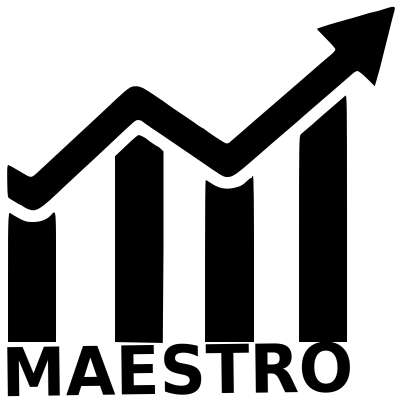
\includegraphics{figures/maestro-logo.pdf}}
        	\end{center}
        \end{figure}
		\end{frame}

		%/////////////////////////////////////////////////
		\section{Motivation}
		\begin{frame}{Motivation}
      \begin{tabular}{cl}
        \begin{tabular}{l}
            \parbox{0.45\linewidth}{%  change the parbox width as appropiate
            \begin{itemize}
            \setlength\itemsep{0.5em}
              \item What is Maestro?
              \vspace{0.5em}
              \begin{itemize}
                  \setlength\itemsep{0.5em}
                  \item Performance tool for \textbf{Message-oriented middleware}.
                  \item Automated, provides reporting.
                  \item Single node, multi node or cluster testing.
              \end{itemize}
              \vspace{0.5em}
              \item Capabilities
              \vspace{0.5em}
              \begin{itemize}
                  \setlength\itemsep{0.5em}
                  \item \textbf{Throughput} measurements.
                  \item \textbf{Latency} measurements.
              \end{itemize}
            \end{itemize}
            }
        \end{tabular}
        & \begin{tabular}{l}
            \scalebox{0.25}{\includegraphics{figures/msg_perf_tool.pdf}}
          \end{tabular} \\
      \end{tabular}
		\end{frame}
		%/////////////////////////////////////////////////
		\section{Extension: Maestro-Agent}
		\begin{frame}{Extensions: Maestro-Agent}
      \begin{tabular}{cl}
        \begin{tabular}{l}
            \parbox{0.55\linewidth}{%  change the parbox width as appropiate
            \begin{itemize}
                \setlength\itemsep{0.5em}
                \item Enables automatic \textbf{SUT} (Software Under Test) changes during the test.
                \item Implements \textbf{Groovy} code handler.
                \item Can fetch and process the \textbf{external repositories}.
                \item The agent tries to execute all scripts in the repository directory.
                \item The repository URL and directory is specified in the test script.
            \end{itemize}
            }
        \end{tabular}
        & \begin{tabular}{l}
            \scalebox{0.40}{\includegraphics{figures/agent_demo.pdf}}
          \end{tabular} \\
      \end{tabular}
		\end{frame}
    %/////////////////////////////////////////////////   
    \section{Extension: AMQP Inspector}
		\begin{frame}{Extensions: AMQP Inspector}
      \begin{itemize}
        \setlength\itemsep{0.5em}
        \item Enables the automatic monitoring of \textbf{Qpid-dispatch} router.
        \item Request-response mechanism over \textbf{AMQP}.
        \item AMQP Inspector sends requests to the \textbf{AMQP Management} continually every few seconds.
        \item AMQP Inspector specification can be changed in the test script.
    \end{itemize}
      \begin{figure}[ht]
        \begin{center}
          \scalebox{0.40}{\includegraphics{figures/inspector_start.pdf}}
        \end{center}
      \end{figure}
    \end{frame}

    %/////////////////////////////////////////////////
		\section{Extension: Topology Generator}
		\begin{frame}{Extension: Topology Generator}
       		\begin{tabular}{cl}
           		\begin{tabular}{l}
             		\parbox{0.55\linewidth}{%  change the parbox width as appropiate
						\begin{itemize}
              \setlength\itemsep{0.5em}
              \item Simplifies the test preparation steps.
              \item Semi-automatic generation of the configuration files for the routers.
							\item Metadata are transformed into variables for the configuration files.
              \begin{itemize}
                \item Inventory
                \item Graph File
              \end{itemize}
							\item Automatic deployment of the configuration files by \textbf{Ansible}.
						\end{itemize}
   					}
         		\end{tabular}
         		& \begin{tabular}{l}
           			\scalebox{0.45}{\includegraphics{figures/generator.pdf}} \\ \\ \\
           		\end{tabular} \\
			\end{tabular}
    \end{frame}
    %/////////////////////////////////////////////////
    \section{Measurements}
    \begin{frame}{Experimental Evaluation}
      \begin{itemize}
          \setlength\itemsep{0.5em}
          \item \textbf{Latency} vs. \textbf{Throughput} vs. \textbf{Behavioral} testing.
          \item The figure shows the throughput and latency comparison of \textbf{Apache ActiveMQ Artemis} and \textbf{Qpid-Dispatch}.
      \end{itemize}
      \begin{figure}[ht]
        \begin{center}
          \scalebox{0.37}{\includegraphics{figures/throughput.pdf}}
          \scalebox{0.37}{\includegraphics{figures/multipoint-latency.pdf}}
        \end{center}
      \end{figure}
    \end{frame}
    %/////////////////////////////////////////////////
		% \section{Measurements II.}
    % \begin{frame}{Experimental Evaluation}
    %   \begin{itemize}
    %       \setlength\itemsep{0.5em}
    %       \item Latency is measured by \textbf{Maestro Receiver}.
    %       \item The figure shows the latency comparison between \textbf{Apache ActiveMQ Artemis} and \textbf{Qpid-Dispatch} connected in a line.
    %   \end{itemize}
    %   \begin{figure}[ht]
    %     \begin{center}
    %       \scalebox{0.7}{\includegraphics{figures/multipoint-latency.pdf}}
    %       % \scalebox{0.4}{\includegraphics{figures/agent.pdf}}
    %     \end{center}
    %   \end{figure}
    % \end{frame}
    %/////////////////////////////////////////////////
    \section{Measurements III.}
    \begin{frame}{Experimental Evaluation with the Agent}
      \begin{itemize}
          \setlength\itemsep{0.5em}
          \item Latency and throughput can be affected by the \textbf{Agent}.
          \item The figure shows the throughput of the several test scenarios with the agent.
      \end{itemize}
      \begin{figure}[ht]
        \begin{center}
          \scalebox{0.7}{\includegraphics{figures/agent-throughput.pdf}}
        \end{center}
      \end{figure}
    \end{frame}
    %/////////////////////////////////////////////////
    \section{Measurements IV.}
    \begin{frame}{Experimental Evaluation with the Agent}
      \begin{itemize}
          \setlength\itemsep{0.5em}
          \item The figure shows behavioral test case, during which one node of the topology is shut down.
      \end{itemize}
      \begin{figure}[ht]
        \begin{center}
          \scalebox{0.7}{\includegraphics{figures/agent-latency.pdf}}
        \end{center}
      \end{figure}
    \end{frame}
		%/////////////////////////////////////////////////
		\section{Summary}
		\begin{frame}{Summary}
				\begin{itemize}
						\setlength\itemsep{0.5em}
						\item Extensions of the Maestro
						\vspace{0.5em}
						\begin{itemize}
							\setlength\itemsep{0.5em}
							\item \textbf{Maestro-Agent}
							\item \textbf{AMQP Inspector}
              \item \textbf{Topology Generator} (external tool)
						\end{itemize}
						\vspace{1em}
						\item Experimental Evaluation
						\vspace{0.5em}
						\begin{itemize}
							\setlength\itemsep{0.5em}
							\item \textbf{Throughput} and \textbf{latency}, \textbf{behavioral} testing.
              \item Single node, multi node or cluster topologies.
              \item Topologies consists of \textbf{Qpid-Dispatch} and \textbf{Apache ActiveMQ Artemis}.
              \item Automatic generation of specific topologies.
						\end{itemize}
				\end{itemize}
		\end{frame}
    %/////////////////////////////////////////////////
    { % these braces make the change local to the single frame
      \setbeamertemplate{footline}
      {
        \leavevmode%
        \hbox{%
        \begin{beamercolorbox}[wd=.3\paperwidth,ht=2.25ex,dp=1ex,center]{author in head/foot}%
          \usebeamerfont{author in head/foot}\insertshortauthor
        \end{beamercolorbox}%
        \begin{beamercolorbox}[wd=.6\paperwidth,ht=2.25ex,dp=1ex,center]{title in head/foot}%
          \usebeamerfont{title in head/foot}\insertshorttitle\hspace*{3em}
        \end{beamercolorbox}}%
        \begin{beamercolorbox}[wd=.1\paperwidth,ht=2.25ex,dp=1ex,center]{date in head/foot}%
          
        \end{beamercolorbox}%
        \vskip0pt%
      }
      \section{Reviewer's Questions}
      \begin{frame}[noframenumbering]{Reviewer's Question}
        \begin{itemize}
            \setlength\itemsep{0.5em}
            \item Jak si vysvětlujete to, že \textbf{Apache ActiveMQ Artemis} má při společném zapojení s \textbf{Qpid-Dispatch} routery větší výkon, než když je zapojen samostatně?
        \end{itemize}
        \begin{figure}[ht]
          \begin{center}
            \scalebox{0.7}{\includegraphics{figures/broker-throughput-comparison.pdf}}
          \end{center}
        \end{figure}
      \end{frame}
    }
    %/////////////////////////////////////////////////
    { % these braces make the change local to the single frame
      \setbeamertemplate{footline}
      {
        \leavevmode%
        \hbox{%
        \begin{beamercolorbox}[wd=.3\paperwidth,ht=2.25ex,dp=1ex,center]{author in head/foot}%
          \usebeamerfont{author in head/foot}\insertshortauthor
        \end{beamercolorbox}%
        \begin{beamercolorbox}[wd=.6\paperwidth,ht=2.25ex,dp=1ex,center]{title in head/foot}%
          \usebeamerfont{title in head/foot}\insertshorttitle\hspace*{3em}
        \end{beamercolorbox}}%
        \begin{beamercolorbox}[wd=.1\paperwidth,ht=2.25ex,dp=1ex,center]{date in head/foot}%
          
        \end{beamercolorbox}%
        \vskip0pt%
      }
      \section{Final Architecture}
      \begin{frame}[noframenumbering]{Final Architecture}
        \begin{figure}[ht]
          \begin{center}
            \scalebox{0.35}{\includegraphics{figures/msg_perf_tool_for_router.pdf}}
          \end{center}
        \end{figure}
      \end{frame}
    }    
    %/////////////////////////////////////////////////
    { % these braces make the change local to the single frame
    \setbeamertemplate{footline}
    {
      \leavevmode%
      \hbox{%
      \begin{beamercolorbox}[wd=.3\paperwidth,ht=2.25ex,dp=1ex,center]{author in head/foot}%
        \usebeamerfont{author in head/foot}\insertshortauthor
      \end{beamercolorbox}%
      \begin{beamercolorbox}[wd=.6\paperwidth,ht=2.25ex,dp=1ex,center]{title in head/foot}%
        \usebeamerfont{title in head/foot}\insertshorttitle\hspace*{3em}
      \end{beamercolorbox}}%
      \begin{beamercolorbox}[wd=.1\paperwidth,ht=2.25ex,dp=1ex,center]{date in head/foot}%
        
      \end{beamercolorbox}%
      \vskip0pt%
    }
    \section{Measurements}
    \begin{frame}[noframenumbering]{Experimental Evaluation Topologies}
      \begin{itemize}
          \setlength\itemsep{0.5em}
          \item Used for \textbf{Latency}, \textbf{Throughput}, \textbf{Behavioral} testing.
          \item The figures shows topologies used for the experimental evaluation.
      \end{itemize}
      \begin{figure}[ht]
        \begin{center}
          \scalebox{0.35}{\includegraphics{figures/basic_topology_router_single.pdf}}
          \scalebox{0.35}{\includegraphics{figures/basic_topology_broker_single.pdf}}
          \scalebox{0.35}{\includegraphics{figures/basic_topology_router.pdf}}
          \scalebox{0.35}{\includegraphics{figures/basic_topology_broker.pdf}}
        \end{center}
      \end{figure}
    \end{frame}
  }

    %/////////////////////////////////////////////////
    { % these braces make the change local to the single frame
      \setbeamertemplate{footline}
      {
        \leavevmode%
        \hbox{%
        \begin{beamercolorbox}[wd=.3\paperwidth,ht=2.25ex,dp=1ex,center]{author in head/foot}%
          \usebeamerfont{author in head/foot}\insertshortauthor
        \end{beamercolorbox}%
        \begin{beamercolorbox}[wd=.6\paperwidth,ht=2.25ex,dp=1ex,center]{title in head/foot}%
          \usebeamerfont{title in head/foot}\insertshorttitle\hspace*{3em}
        \end{beamercolorbox}}%
        \begin{beamercolorbox}[wd=.1\paperwidth,ht=2.25ex,dp=1ex,center]{date in head/foot}%
          
        \end{beamercolorbox}%
        \vskip0pt%
      }
      \section{Measurements III. v2}
      \begin{frame}[noframenumbering]{Agent Topology}
        \begin{itemize}
            \setlength\itemsep{0.5em}
            \item The topology used for the behavioral testing and analysis.
        \end{itemize}
        \begin{figure}[ht]
          \begin{center}
            \scalebox{0.45}{\includegraphics{figures/basic_topology_router_agent_redundant.pdf}}
          \end{center}
        \end{figure}
      \end{frame}
    }
    %/////////////////////////////////////////////////
    % \section{Contacts}
    % \begin{frame}[noframenumbering]{Contacts}
    %   \begin{figure}[ht]
    %     \begin{center}
    %       \scalebox{0.30}{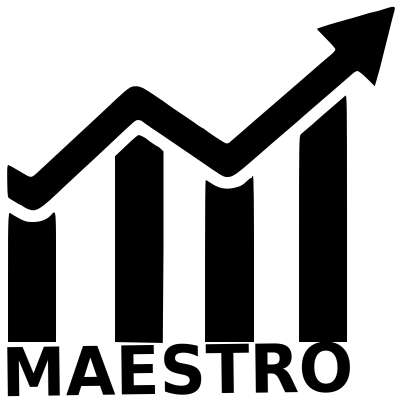
\includegraphics{figures/maestro-logo.pdf}}
    %     \end{center}
    %   \end{figure}
    %   \begin{center}
    %     \begin{itemize}
    %       \item Jakub Stejskal\,---\,jstejska@redhat.com, xstejs24@stud.fit.vutbr.cz
    %       \item Otavio Rudolfo Piske\,---\,opiske@redhat.com (Author of Maestro)
    %       \item GitHub\,---\,\url{https://github.com/maestro-performance/}
    %     \end{itemize}
    % \end{center}
    % \end{frame}
    %/////////////////////////////////////////////////

\end{document}
